In diesem Kapitel werden alle Arten der Plots einmal vorgestellt und auf alle Eigenheiten eingegangen, damit diese verstanden werden. 

Es wird hier sowohl auf die Achsenbeschriftung als auch auf die Texte innerhalb der Plots eingegangen. 

\begin{figure}[htpb]
    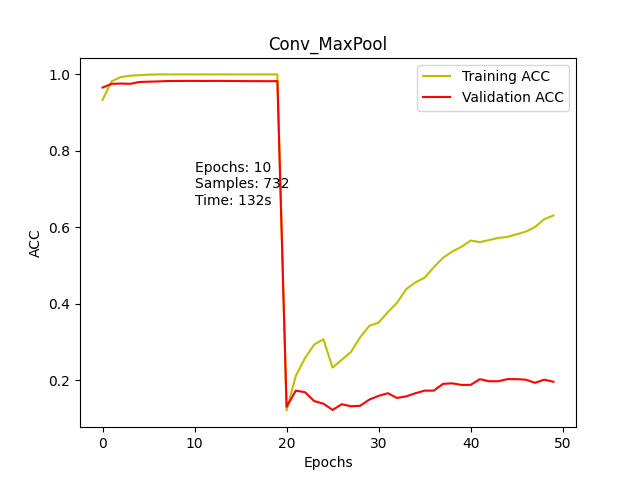
\includegraphics[height=5cm]{../../Plots/ba_plots/convmaxpool/2TFtr.png}
    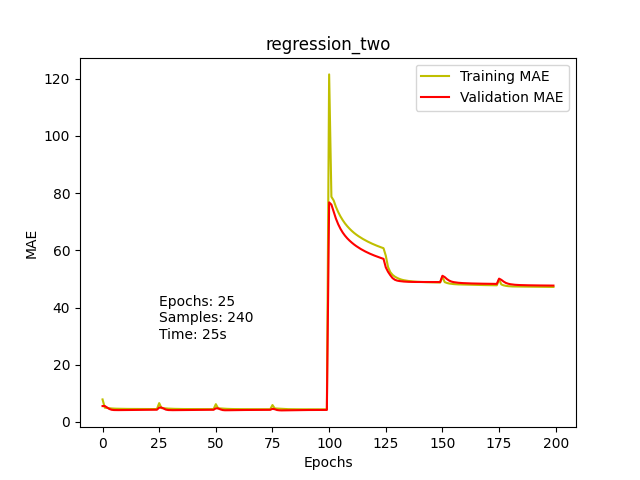
\includegraphics[height=5cm]{../../Plots/ba_plots/regr2/regr2train.png}
    \caption{\label{fig:ploterkl} Vorstellung Plots}
\end{figure}

Dazu wird Figure 3.1 betrachtet. In beiden Teilen stehen drei Zeilen Text auf die nun einzelnd eingegangen wird. Die Erste sagt aus, 
wieviele Epochen pro Layer oder Netzwerk trainiert worden sind. Die Zweite beschreibt wieviele Datensamples des Trainingssets des 
Targetdatensatzes im Training nach TF genutzt worden sind und die dritte Zeile zeigt die gesamte Trainingsdauer in Sekunden an. 

Wenn es um die Accuracy geht, was bei Klassifikation der Fall ist, dann steht ACC auf der senkrechten Achse und beim Funktionsnamen dabei. 
Die senkrechte Achse ist dann bei 100\%, wenn sie bei 1 ist. In Figure 3.1 ist links ein Beispielplot für diesen Fall. 

Für die Regression, geht es um den MAE. Dies steht wiederum in den Namen der Funktionen und der senkrechten Achse. Diese Achse ist in 1000\$ pro 
Einheit. Dabei ist es besser, je geringer der Wert ist. 
